\chapter{FUNCIONES DE VARIAS VARIABLES}
%\startcontents
\printchaptertableofcontents

El estudio de las funciones de varias variables constituye un pilar fundamental en el ámbito del Cálculo III, donde se exploran fenómenos matemáticos que implican más de una dimensión. A diferencia del cálculo de una sola variable, donde las funciones dependen únicamente de un parámetro, en el cálculo de varias variables, las funciones pueden depender de dos o más variables independientes. Este capítulo se adentra en la comprensión y análisis de estas funciones, explorando su comportamiento, propiedades y aplicaciones en diversos contextos.

En esencia, una función de varias variables asigna a cada punto en un dominio de dos o más dimensiones un único valor en el espacio real. Este enfoque multifacético permite modelar y comprender una amplia gama de fenómenos físicos, económicos y científicos, desde la trayectoria de un proyectil en el espacio hasta la distribución de temperatura en un sólido tridimensional.

La comprensión de las funciones de varias variables requiere el dominio de conceptos clave, entre ellos, la noción de dominio y rango, continuidad, derivadas parciales, gradientes, y optimización. A través del análisis de estas herramientas matemáticas, los estudiantes desarrollarán una perspicacia profunda sobre cómo las funciones de varias variables se comportan y cómo pueden ser utilizadas para resolver problemas prácticos.

Este capítulo se estructura para guiar al lector desde los conceptos básicos hasta las aplicaciones avanzadas. Comienza con la definición formal de una función de varias variables, examinando su representación gráfica y sus propiedades fundamentales. A medida que avanzamos, exploramos la diferenciabilidad y la integrabilidad de estas funciones, así como las técnicas para encontrar máximos y mínimos locales y absolutos.

%Además, se abordan aplicaciones relevantes en campos como la física, la ingeniería, la economía y las ciencias computacionales, ilustrando cómo las funciones de varias variables se utilizan para modelar situaciones del mundo real y resolver problemas complejos.

\section{Funciones y su dominio}

\begin{definition}
    Una función $f$ de dos variables es una regla que asigna a cada par ordenado de números reales $(x, y)$ de un conjunto $D$, un único número real que se denota con $f(x, y)$. El conjunto $D$ es el dominio de $f$ y su rango es el conjunto de valores que toma $f$, es decir, $\left\{ f(x, y) \mid (x, y) \in D \right\}$.
\end{definition}

A menudo, escribimos $z = f(x, y)$ para hacer explícito el valor que toma $f$ en el punto $(x, y)$. Las variables $x$ y $y$ son variables independientes y $z$ es la variable dependiente [compare lo anterior con la notación $y = f(x)$ para funciones de una variable].
\sideFigure[\label{fig:Funcion_dos_variables}]{
    \centering
    \includegraphics[width=\linewidth]{Images/Capitulo1/Funcion_dos_variables.pdf}
}

Una función de dos variables es una función cuyo dominio es un subconjunto de $\mathbb{R}^2$ y cuyo rango es un subconjunto de $\mathbb{R}$. Una manera de representar tal función es mediante un diagrama de flechas (véase la figura \ref{fig:Funcion_dos_variables}), donde el dominio $D$ se representa como un subconjunto del plano $x y$ y el rango es un conjunto de números sobre una recta real, que se muestra como un eje $z$. %Por ejemplo, si $f(x, y)$ representa la temperatura en un punto $(x, y)$ en una placa metálica plana con la forma de $D$, podemos considerar al eje $z$ como un termómetro que va mostrando el registro de temperaturas.

Si una función $f$ está dada por una fórmula y no se especifica dominio alguno, entonces se entiende que el dominio de $f$ será el conjunto de parejas $(x, y)$ para el cual la expresión dada es un número bien definido.

\begin{example}
    Para las siguientes funciones, evalúe $f(3, 2)$ y determine y grafique el dominio.
    \begin{tasks}(2)
        \task $\displaystyle f(x, y) = \frac{\sqrt{x + y + 1}}{x - 1}$
        \task $f(x, y) = x \ln (y^2 - x)$
    \end{tasks}
    \solucion
    \begin{enumerate}[label=\alph*)]
        \item Tenemos que\sideFigure[\label{Fig:Dominio_1}Representación geométrica del dominio de $\displaystyle f(x, y) = \frac{\sqrt{x + y + 1}}{x - 1}$]{
        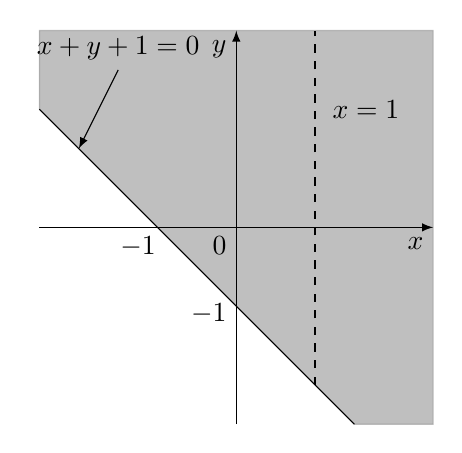
\begin{tikzpicture}
            \filldraw[gray,opacity=0.5] (1.5,-2.5) --(2.5,-2.5) -- (2.5,2.5) -- (-2.5,2.5) -- (-2.5,1.5) -- (1.5,-2.5) -- cycle;
            \draw[-latex] (-2.5,0) -- (2.5,0) node[below left] {$x$};
            \draw[-latex] (0,-2.5) -- (0,2.5) node[below left] {$y$};
            \draw (-2.5,1.5) -- (1.5,-2.5);
            \draw[latex-] (-2,1) -- (-1.5,2) node[above] {$x + y + 1 = 0$};
            \node[below left] at (0,0) {$0$};
            \node[below left] at (-0.9,0) {$-1$};
            \node[left] at (0,-1.1) {$-1$};
            \draw[dash pattern=on 3pt off 3pt] (1,-2) -- (1,2.5);
            \node[right] at (1.1,1.5) {$x = 1$};
        \end{tikzpicture}
        }
        $$f(3, 2) = \frac{\sqrt{3 + 2 + 1}}{3 - 1} = \frac{\sqrt{6}}{2}$$
        La expresión para $f$ tiene sentido si el denominador no es cero y la cantidad dentro del signo de raíz cuadrada es no negativa. Entonces, el dominio de $f$ es
        $$D = \left\{ (x, y) \in \RR[2] \mid x + y + 1 \geq 0, x \neq 1 \right\}.$$
        La desigualdad $x + y + 1 \geq 0$, o bien, $y \geq -x - 1$, describe los puntos que quedan en o por arriba de la recta $y = -x - 1$, mientras que $x \neq 1$ significa que los puntos sobre la recta $x = 1$ tienen que ser excluidos del dominio. Vea la figura \ref{Fig:Dominio_1}.
        \item Tenemos que\sideFigure[\label{Fig:Dominio_2}Representación geométrica del dominio de $f(x, y) = x \ln (y^2 - x)$]{
        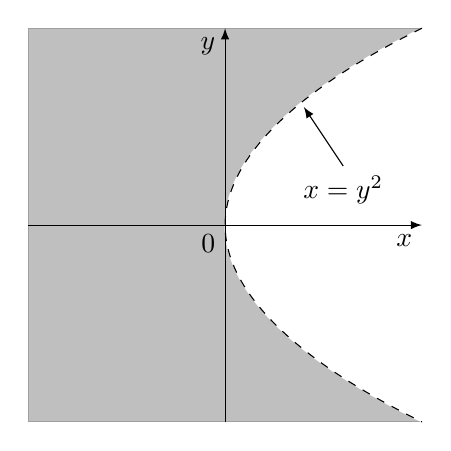
\begin{tikzpicture}
            \filldraw[gray,opacity=0.5] (-2.5,-2.5) rectangle (2.49,2.5);
            \node[below left] at (0,0) {$0$};
            \filldraw[rotate=-90,white] (-2.5,2.5) parabola bend (0,0) (2.5,2.5);
            \draw[rotate=-90,dash pattern=on 3pt off 3pt] (-2.5,2.5) parabola bend (0,0) (2.5,2.5);
            \draw[latex-] (1,1.5) -- (1.5,0.75) node[below] {$x = y^2$};
            \draw[-latex] (-2.5,0) -- (2.5,0) node[below left] {$x$};
            \draw[-latex] (0,-2.5) -- (0,2.5) node[below left] {$y$};
        \end{tikzpicture}
        }
        $$f(3, 2) = 3 \ln (2^2 - 3) = 0.$$
        Puesto que $\ln(y^2 - x)$ se define solo cuando $y^2 - x > 0$, es decir, $x < y^2$, el dominio de $f$ es
        $$D = \left\{ (x, y) \in \RR[2] \mid x < y^2 \right\}.$$
        Este es el conjunto de puntos a la izquierda de la parábola $x = y^2$. Vea la figura \ref{Fig:Dominio_2}.
    \end{enumerate}
\end{example}

\begin{example}
    Determine y grafique el dominio de las siguientes funciones:
    \begin{tasks}(2)
        \task $f(x, y) = \sqrt{x^2 + y^2 - 1}$
        \task $f(x, y) = \ln (x^2 + y^2 - 1)$
    \end{tasks}
    \newpage
    \solucion \sideFigure[\label{Fig:Dominio_3}Representación geométrica del dominio de $f(x, y) = \sqrt{x^2 + y^2 - 1}$]{
    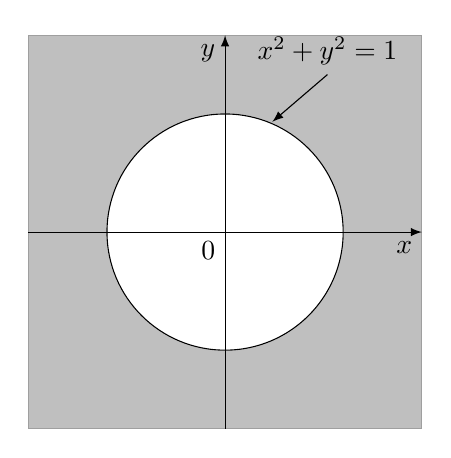
\begin{tikzpicture}
        \filldraw[gray,opacity=0.5] (-2.5,-2.5) rectangle (2.5,2.5);
        \filldraw[white] (0,0) circle (1.5cm);
        \draw (0,0) circle (1.5cm);
        \draw[-latex] (-2.5,0) -- (2.5,0) node[below left] {$x$};
        \draw[-latex] (0,-2.5) -- (0,2.5) node[below left] {$y$};
        \node[below left] at (0,0) {$0$};
        \draw[latex-] (0.6,1.4) -- (1.3,2) node[above] {$x^2 + y^2 = 1$};
    \end{tikzpicture}
    }
    \begin{enumerate}[label=\alph*)]
        \item Siguiendo la misma idea el ejemplo anterior, la expresión para $f$ tiene sentido si la cantidad dentro del signo de raíz cuadrada es no negativa. Así, el dominio de $f$ es
        $$D = \left\{ (x, y) \in \RR[2] \mid x^2 + y^2 - 1 \geq 0 \right\}.$$
        La desigualdad $x^2 + y^2 - 1 \geq 0$, o bien, $x^2 + y^2 \geq 1$, describe los puntos que quedan en o fuera de la circunferencia $x^2 + y^2 = 1$.
        \item Puesto que $\ln (x^2 + y^2 - 1)$ se define solo cuando $x^2 + y^2 - 1 > 0$, es decir, $x^2 + y^2 > 1$ el dominio de $f$ es\sideFigure[\label{Fig:Dominio_4}Representación geométrica del dominio de $f(x, y) = \ln (x^2 + y^2 - 1)$]{
        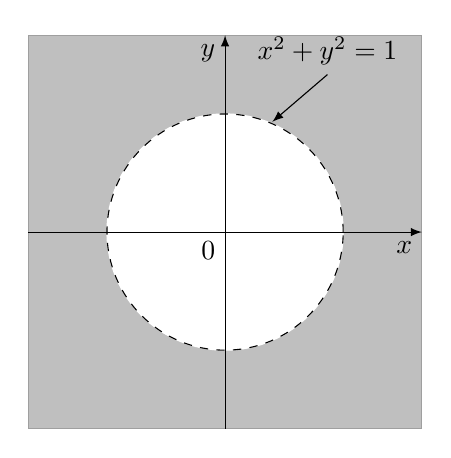
\begin{tikzpicture}
            \filldraw[gray,opacity=0.5] (-2.5,-2.5) rectangle (2.5,2.5);
            \filldraw[white] (0,0) circle (1.5cm);
            \draw[dash pattern=on 3pt off 3pt] (0,0) circle (1.5cm);
            \draw[-latex] (-2.5,0) -- (2.5,0) node[below left] {$x$};
            \draw[-latex] (0,-2.5) -- (0,2.5) node[below left] {$y$};
            \node[below left] at (0,0) {$0$};
            \draw[latex-] (0.6,1.4) -- (1.3,2) node[above] {$x^2 + y^2 = 1$};
        \end{tikzpicture}
        }
        $$D = \left\{ (x, y) \in \RR[2] \mid x^2 + y^2 > 1 \right\}.$$
        Este es el conjunto de puntos que están fuera de la circunferencia sin tomar los puntos que están en $x^2 + y^2 = 1$.
    \end{enumerate}
\end{example}

\begin{definition}
    Una función de tres variables, $f$, es una regla que asigna a cada terna ordenada $(x, y, z)$ en un dominio $D \subseteq \RR[3]$ un único número real denotado por $f(x, y, z)$.
\end{definition}

\begin{example}
    Graficar el dominio de la siguiente función:
    $$f(x, y, z) = \sqrt{x^2 + y^2 + z^2 - 4} + \ln \left( \frac{1}{\sqrt{x^2 + y^2 -1}} \right).$$
    \solucion Procediendo como ejemplos anteriores, notemos que se debe cumplir que
    $$x^2 + y^2 + z^2 - 4 \geq 0 \quad \text{ y } \quad x^2 + y^2 - 1 > 0.$$
    Analicemos la primer desigualdad, si tomamos la igualdad, obtenemos
    \begin{align*}
        x^2 + y^2 + z^2 - 4 & \geq 0 \\
        x^2 + y^2 + z^2 & \geq 4
    \end{align*}
    la cual es una esfera centrada en el origen y de radio igual a $2$. Luego, tomando la segunda desigualdad, se sigue que
    \begin{align*}
        x^2 + y^2 - 1 & > 0 \\
        x^2 + y^2 & > 1
    \end{align*}
    Si se toma la igualdad, esta será un cilindro de radio igual a $1$. Así, el dominio de la función $f$ es todo el exterior tanto del cilindro, como de la esfera. La función puede tomar puntos del “contorno” de la esfera, pero no puede tomar puntos del “contorno” del cilindro. Es difícil dibujar con exactitud el dominio de $f$, pero puede mirar la figura \ref{funcion3d}.\sideFigure[\label{funcion3d}]{
    \includegraphics[width=\linewidth]{Images/Capitulo1/Dominio_de_funcion3d.pdf}
    }
\end{example}

\begin{example}
    Graficar el dominio de la siguiente función:
    $$f(x, y, z) = \sqrt{x^2 + y^2 - 4} + \frac{1}{y + z - 2}.$$
    \solucion Procediendo como ejemplos anteriores, notemos que se debe cumplir que
    $$x^2 + y^2 - 4 \geq 0 \quad \text{ y } \quad y + z - 2 \neq 0.$$
    Analicemos la primer desigualdad, si tomamos la igualdad, obtenemos\sideFigure[\label{dominiodefuncion3d}]{
    \includegraphics[width=\linewidth]{Images/Capitulo1/Dominio_de_funcion_en3D.pdf}
    }
    \begin{align*}
        x^2 + y^2 - 4 & \geq 0 \\
        x^2 + y^2 & \geq 4
    \end{align*}
    la cual es un cilindro centrado en el origen y de radio igual a $2$. Luego, analizando la segunda expresión; si tomamos la igualdad, se obtiene $y + z = 2$, el cual, es un plano. Por lo tanto, el dominio de $f$ es el conjunto de $(x, y, z)$ que quedan en o fuera del cilindro $x^2 + y^2 = 4$. Además, no puede tomar los puntos que conforma el plano $y + z - 2 = 0$, pues la división entre $0$ no está definida. Es difícil dibujar con exactitud el dominio de $f$, pero puede mirar la figura \ref{dominiodefuncion3d}.
\end{example}

\section{Gráficas de funciones y curvas de nivel}

\begin{reminder}
    Es importante destacar que el círculo es un caso particular de la elipse, pues recordemos que la expresión para una circunferencia centrada en el origen está dada por
    $$x^2 + y^2 = r^2$$
    donde $r$ es el radio de dicha circunferencia y es una constante real, mientras que una elipse está dada por
    $$\frac{x^2}{a^2} + \frac{y^2}{b^2} = 1$$
    siendo $a$ y $b$ constantes reales. Generalmente la elipse tiene dos ejes de diferentes longitudes y dos focos distintos, pero el círculo es una forma particular de elipse donde ambos ejes son idénticos y los dos focos coinciden en el centro del círculo. La elipse puede presentarse de dos maneras distintas: horizontalmente o verticalmente. Cuando decimos que una elipse está en posición horizontal, significa que su eje mayor se extiende más en el eje $x$, mientras que en la posición vertical, el eje mayor se extiende más en el eje $y$.
    \begin{figure}[h!]
        \centering
        \subfloat[Elipse horizontal: Cuando $a>b$]{
        \begin{tikzpicture}[scale=0.9]
            \draw[-latex] (-3,0) -- (3,0) node[below left] {$x$};
            \draw[-latex] (0,-3) -- (0,3) node[below left] {$y$};
            \draw (0,0) ellipse (2cm and 1cm);
        \end{tikzpicture}
        } \hfill
        \subfloat[Elipse vertical: Cuando $b>a$]{
        \begin{tikzpicture}[scale=0.9]
            \draw[-latex] (-3,0) -- (3,0) node[below left] {$x$};
            \draw[-latex] (0,-3) -- (0,3) node[below left] {$y$};
            \draw (0,0) ellipse (1cm and 2cm);
        \end{tikzpicture}
        }
        \caption{Representación de la elipse}
    \end{figure}
    
    \noindent La hipérbole es otra cónica, al igual que la elipse. Sin embargo, a diferencia de la elipse que tiene una forma cerrada, la hipérbole es una curva abierta que se extiende hacia el infinito en ambas direcciones. En términos algebraicos, la ecuación de una hipérbole con centro en el origen se expresa como:
    $$\frac{x^2}{a^2} - \frac{y^2}{b^2} = 1$$
    donde $a$ y $b$ son constantes reales. Al igual que la elipse, la hipérbole puede presentarse en dos configuraciones principales: horizontal y vertical. En el caso de una hipérbole horizontal, las ramas principales de la hipérbole se extienden horizontalmente a lo largo del eje $x$, mientras que en una hipérbole vertical, las ramas principales se extienden verticalmente a lo largo del eje $y$.
    \begin{figure}[h!]
        \centering
        \subfloat[Hipérbole horizontal: Cuando $a>b$]{
        \begin{tikzpicture}[scale=0.9]
            \draw[-latex] (-3,0) -- (3,0) node[below left] {$x$};
            \draw[-latex] (0,-3) -- (0,3) node[below left] {$y$};
            \draw[rotate=90,yshift=1cm] (-2,2) parabola bend (0,0) (2,2);
            \draw[rotate=-90,yshift=1cm] (-2,2) parabola bend (0,0) (2,2);
        \end{tikzpicture}
        } \hfill
        \subfloat[Hipérbole vertical: Cuando $b>a$]{
        \begin{tikzpicture}[scale=0.9]
            \draw[-latex] (-3,0) -- (3,0) node[below left] {$x$};
            \draw[-latex] (0,-3) -- (0,3) node[below left] {$y$};
            \draw[yshift=1cm] (-2,2) parabola bend (0,0) (2,2);
            \draw[rotate=180,yshift=1cm] (-2,2) parabola bend (0,0) (2,2);
        \end{tikzpicture}
        }
        \caption{Representación de la hipérbole}
    \end{figure}
\end{reminder}
%Otro modo de visualizar el comportamiento de una función de dos variables es considerar su gráfica

\sideFigure[\label{fig:1.6defuncion}]{\vspace{2cm}
\tdplotsetmaincoords{75}{110}
\begin{tikzpicture}[tdplot_main_coords,scale=2]
    \draw[thick,-latex] (0,0,0) coordinate(O) -- (2.5,0,0) node[anchor=north east] (x) {$x$};
    \draw[thick,-latex] (0,0,0) -- (0,1.5,0) node[anchor=north west] (y) {$y$};
    \draw[thick,-latex] (0,0,0) -- (0,0,2.5) node[anchor=south] (z) {$z$};
    \begin{scope}[xshift=0mm,rotate=-10]
        \tikzfading[name=fade right,
            left color=transparent!00,
            right color=transparent!60] ;
            \filldraw[black!30,path fading=fade right,fill opacity=0.5,
            ]  plot[variable=\x,samples=180,domain=-90:270] ({1.2*cos(\x)},{sin(\x)},{0});
            \draw plot[variable=\x,samples=180,domain=-90:270] ({1.2*cos(\x)},{sin(\x)},{0});
    \end{scope}
    \coordinate[label={[name=Plabel,xshift=0.5cm,yshift=1.7cm]above right:{$\big(x, y, f(x, y)\big)$}}] (P) at (0.2,0.5,1.2);
    \draw[-latex,shorten >=2.5pt] (Plabel) --(P);
    \fill (P) circle (1pt);
    \coordinate[label=below:{$(x, y, 0)$}] (Q) at (0.2,0.5,0);
    \fill (Q) circle (1pt);
    \draw[thick,] (P) -- (Q);
    \draw[thick,decoration={brace,raise=2.5pt},decorate] (P) -- (Q) node[midway,right=2mm]{$f(x, y)$};
    \draw[fill=gray,fill opacity=0.5,name path=back,->] plot[variable=\x,samples=180,domain=50:270] ({1.2*cos(\x)},{sin(\x)},{1.2+0.4*cos(2*\x)}) to[out=30,in=160] cycle;
    \draw[fill=gray,fill opacity=0.5,name path=front] plot[variable=\x,samples=180,domain=-90:50] ({1.2*cos(\x)},{sin(\x)},{1.2+0.4*cos(2*\x)}) to[out=160,in=30] cycle;
    \node[xshift=-0.2cm,yshift=1cm] at (0.2,0.5,1.2) {$S$};
    \node[xshift=-1.5cm,yshift=0.2cm] at (0.2,0.5,0) {$D$};
\end{tikzpicture}
}

\sideFigure[Un ejemplo común de las curvas de nivel son los mapas topográficos de regiones montañosas]{
\includegraphics[width=\linewidth]{Images/Capitulo1/Cartografico.pdf}
}
\sideFigure[\label{fig:curvasdenivelre}Representación geométrica de las curvas de nivel de una función]{
\includegraphics[width=\linewidth]{Images/Capitulo1/Curvas_de_nivelBW.pdf}
}
\vspace{-0.5cm}
\begin{definition}
    Sea $f:D \subseteq \RR[n] \longrightarrow \RR$ una función, entonces la gráfica de $f$ es
    $$\mathcal{G}(f) = \left\{ \big(x, f(x)\big) \mid x \in D \right\} \subseteq \RR[n+1].$$
\end{definition}

\begin{observation}
    Si $f$ es una función de dos variables con dominio $D$, entonces la gráfica de $f$ es el conjunto de todos los puntos $(x, y, z)$ en $\RR[3]$ tal que $(x, y)$ y $z = f(x, y)$ está en $D$.
\end{observation}

Así como la gráfica de una función $f$ de una variable es una curva $C$ con ecuación $y = f (x)$, la gráfica de una función $f$ de dos variables es una superficie $S$ cuya ecuación es $z = f (x, y)$. Podemos visualizar la gráfica $S$ de $f$ directamente sobre o abajo de su dominio $D$ en el plano $xy$ (véase la figura \ref{fig:1.6defuncion}).

Un método para poder graficar funciones de dos funciones es mediante un mapa de curvas de nivel en el cual puntos de elevación igual se unen para formar líneas de contorno o curvas de nivel. Las curvas de nivel son líneas imaginarias que se utilizan para representar superficies tridimensionales en dos dimensiones, como mapas topográficos o gráficos de funciones de dos variables. Estas curvas conectan puntos que tienen la misma altura o el mismo valor de la función en el caso de las superficies. Por ejemplo, en un mapa topográfico, las curvas de nivel unen puntos que tienen la misma elevación sobre el nivel del mar. Al observar estas curvas, podemos entender la variación de la elevación o la función en diferentes áreas de la superficie, lo que proporciona una representación visual y comprensible del terreno o de la función en cuestión. %Las curvas de nivel son una herramienta poderosa en diversas áreas, desde la cartografía hasta la ingeniería y las ciencias ambientales, facilitando la interpretación y el análisis de datos espaciales y funcionales.

\begin{definition}
    Se define la \textbf{curva de nivel} de $f$ correspondiente al valor $k \in \RR$ como
    $$\mathcal{C}_k(f) = \left\{ (x_1, x_2, \dots, x_n) \in D \mid f(x_1, x_2, \dots, x_n) = k \right\}.$$
\end{definition}

\begin{observation}
    Una curva de nivel $f(x, y) = k$ es el conjunto de todos los puntos en el dominio de $f$ en el cual $f$ toma un valor dado $k$. En otras palabras, señala dónde tiene una altura $k$ la gráfica de $f$. Vea la imagen \ref{fig:curvasdenivelre}.
\end{observation}

\begin{example}
    Graficar la función $f(x, y) = x^{2} - y^{2}$.\\
    \solucion Para graficar la función $f$, obtengamos algunas curvas de nivel. Sea $z = x^2 - y^2$,
    \begin{itemize}
        \item Si $z = 0$, entonces
        \begin{align*}
            0 & = x^2 - y^2 \\
            & = (x-y)(x+y);
        \end{align*}
        así que $y = x$ o $y = -x$. Es decir, obtenemos dos rectas perpendiculares.
        \item Si $z = 1$, entonces
        $$1 = x^2 - y^2;$$
        así que obtenemos una hipérbole (cuando $y = 0$, $x = \pm 1$).
        \item Si $z = 2$, entonces
        $$2 = x^2 - y^2;$$
        así que obtenemos una hipérbole (cuando $y = 0$, $x = \pm \sqrt{2}$).
        \item Si $z = 3$, entonces
        $$3 = x^2 - y^2;$$
        así que obtenemos una hipérbole (cuando $y = 0$, $x = \pm \sqrt{3}$).
    \end{itemize}
    Entonces, las curvas de nivel (en el plano $xy$) son como se muestran a continuación:
    \begin{figure}[h!]
        \centering
        \subfloat[Cuando $z = 0$]{
        \begin{tikzpicture}
            \draw[-latex] (-2.5,0) -- (2.5,0) node[below left] {$x$};
            \draw[-latex] (0,-2.5) -- (0,2.5) node[below left] {$y$};
            \draw (-2.5,-2.5) -- (2.5,2.5);
            \draw (-2.5,2.5) -- (2.5,-2.5);
        \end{tikzpicture}
        } \hfill
        \subfloat[Cuando $z = 1$]{
        \begin{tikzpicture}
            \draw[-latex] (-2.5,0) -- (2.5,0) node[below left] {$x$};
            \draw[-latex] (0,-2.5) -- (0,2.5) node[below left] {$y$};
            \draw[rotate=90,yshift=0.5cm] (-2,2) parabola bend (0,0) (2,2);
            \draw[rotate=-90,yshift=0.5cm] (-2,2) parabola bend (0,0) (2,2);
            \node[below] at (-1,0) {$-1$};
            \node[below] at (1,0) {$1$};
        \end{tikzpicture}
        } \\
        \subfloat[Cuando $z = 2$]{
        \begin{tikzpicture}
            \draw[-latex] (-2.5,0) -- (2.5,0) node[below left] {$x$};
            \draw[-latex] (0,-2.5) -- (0,2.5) node[below left] {$y$};
            \draw[rotate=90,yshift=0.7cm] (-2,1.8) parabola bend (0,0) (2,1.8);
            \draw[rotate=-90,yshift=0.7cm] (-2,1.8) parabola bend (0,0) (2,1.8);
            \node[below] at (-1.2,0) {$-\sqrt{2}$};
            \node[below] at (1.2,0) {$\sqrt{2}$};
        \end{tikzpicture}
        } \hfill
        \subfloat[Cuando $z = 3$]{
        \begin{tikzpicture}
            \draw[-latex] (-2.5,0) -- (2.5,0) node[below left] {$x$};
            \draw[-latex] (0,-2.5) -- (0,2.5) node[below left] {$y$};
            \draw[rotate=90,yshift=0.86cm] (-2,1.6) parabola bend (0,0) (2,1.6);
            \draw[rotate=-90,yshift=0.86cm] (-2,1.6) parabola bend (0,0) (2,1.6);
            \node[below] at (-1.4,0) {$-\sqrt{3}$};
            \node[below] at (1.4,0) {$\sqrt{3}$};
        \end{tikzpicture}
        }
        \caption{Algunas curvas de nivel de $x^2 - y^2$}
    \end{figure}
    \newpage
    \noindent Por último, encontremos los “perfiles” de la función. Si $y = 0$, entonces $z = x^2$; y si $x = 0$, entonces $z = -x^2$. Por tanto, la gráfica de la función $f(x, y) = x^{2} - y^{2}$ está dada como sigue:
    \begin{figure}[h!]
        \centering
        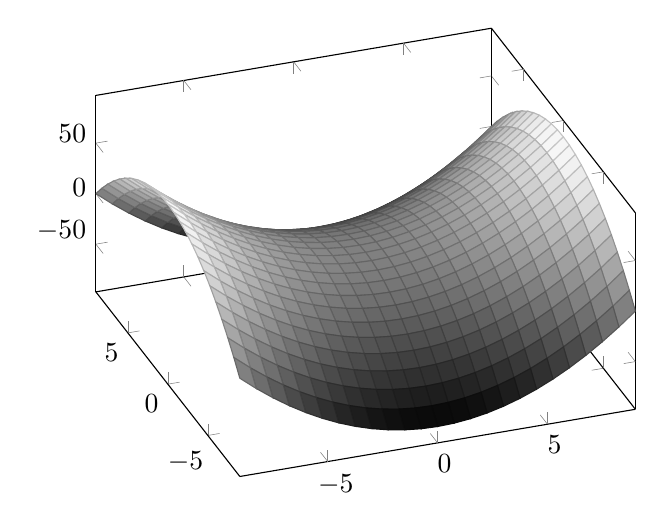
\begin{tikzpicture}
            \begin{axis}[view={-20}{45},
                %axis lines=center,
                %axis on top,
                colormap/blackwhite
                ]
                \addplot3 [surf,
                draw=black,
                domain=-9:9,
                domain y=-9:9,
                ] {x^2-y^2};
            \end{axis}
        \end{tikzpicture}
        \caption{Gráfica de la función $x^2 - y^2$}
    \end{figure}
\end{example}

\section{Definición y ejemplos de normas}

Una norma en el contexto del cálculo de varias variables es una función que asigna a cada vector en un espacio vectorial una magnitud no negativa, de modo que satisface ciertas propiedades fundamentales. La norma más comúnmente utilizada es la norma euclidiana o norma $\ell_2$, que se define como la raíz cuadrada de la suma de los cuadrados de las componentes del vector. Esta norma captura la noción geométrica de distancia y es fundamental en el análisis vectorial y el cálculo diferencial e integral.

Además de la norma euclidiana, existen otras normas importantes en el cálculo de varias variables, como la norma $\ell_1$ (que es la suma de los valores absolutos de las componentes del vector), la norma $\ell_{\infty}$ (que es el máximo valor absoluto de las componentes del vector), entre otras.

\begin{definition}
    Sea $V$ un espacio vectorial sobre $K$ (donde $K$ generalmente es el conjunto de los números reales $\mathbb{R}$ o los números complejos $\mathbb{C}$). La norma en $V$ es una función $\| \quad \| : V \longrightarrow \RR$ que satisface las siguientes propiedades: Para todo $\mathbf{x}$, $\mathbf{y} \in V$ y $\lambda \in K$
    \begin{enumerate}[label=\roman*.]
        \item $\| \mathbf{x} \| \geq 0$,
        \item $\| \mathbf{x} \| = 0$ si y solo si $\mathbf{x} = \mathbf{0}$,
        \item $\| \lambda \mathbf{x} \| = |\lambda| \| \mathbf{x} \|$,
        \item $\| \mathbf{x} + \mathbf{y} \| \leq \| \mathbf{x} \| + \| \mathbf{y} \|$ (desigualdad del triángulo).
    \end{enumerate}
\end{definition}

\begin{example}
    En $\RR$, sea $\| \mathbf{x} \| = |x|$, probemos entonces que $\| \quad \|$ cumple las cuatro propiedades establecidas en la definición previa.
    \begin{enumerate}[label=\roman*.]
        \item Sea $\mathbf{x} \in \RR$, entonces
        \begin{align*}
            \| \mathbf{x} \| & = |x| \\
            & \geq 0 
        \end{align*}
        Por tanto, $\| \mathbf{x} \| \geq 0$.
        \item Por el curso de Cálculo I,
        $$\| \mathbf{x} \| = 0_{\RR} \Longleftrightarrow |x| = 0_{\RR} = 0 \Longleftrightarrow x = 0 = \mathbf{0}_V.$$
        Por tanto, $\| \mathbf{x} \| = 0$ si y solo si $\mathbf{x} = \mathbf{0}$.
        \item Sea $\mathbf{x} \in \RR$ y $\lambda \in \RR$, entonces
        \begin{align*}
            \| \lambda \mathbf{x} \| & = |\lambda x| \\
            & = |\lambda| |x| \\
            & = |\lambda| \| \mathbf{x} \| 
        \end{align*}
        Por tanto, $\| \lambda \mathbf{x} \| = |\lambda| \| \mathbf{x} \|$.
        \item Sean $\mathbf{x}$, $\mathbf{y} \in \RR$, entonces
        \begin{align*}
            \| \mathbf{x} + \mathbf{y} \| & = |x + y| \\
            & \leq |x| + |y| \\
            & = \| \mathbf{x} \| + \| \mathbf{y} \|
        \end{align*}
        Por tanto, $\| \mathbf{x} + \mathbf{y} \| \leq \| \mathbf{x} \| + \| \mathbf{y} \|$.
    \end{enumerate}
    Dado que $\| \quad \|$ satisface las cuatro propiedades de una norma, concluimos que  $\| \quad \|$ es una norma.
\end{example}

\begin{observation}
    En el ejemplo anterior, aunque el espacio vectorial era $\RR$, es importante distinguir entre los vectores y los números reales, pues son cosas muy distintas. Por tanto, los vectores los representaremos utilizando letras en negrita para distinguirlos de los números reales.
\end{observation}

\begin{example}
    En $\RR[2]$, sea $\| (x, y) \|_1 = |x| + |y|$, probemos entonces que $\| \quad \|_1$ cumple las cuatro propiedades establecidas en la definición previa.
    \begin{enumerate}[label=\roman*.]
        \item Sea $(x, y) \in \RR[2]$, entonces
        \begin{align*}
            \| (x, y) \|_1 & = \smallunderbrace{|x|}_{\geq 0} + \smallunderbrace{|y|}_{\geq 0} \\
            & \geq 0
        \end{align*}
        Así, $\| (x, y) \|_1 \geq 0$.
        \item \begin{enumerate}
            \item[$\Rightarrow)$] Sea $(x, y) \in \RR[2]$, entonces
            $$\| (x, y) \|_1 = |x| + |y|,$$
            así que $|x| = 0$ y $|y| = 0$. Es decir, $x = 0$ y $y = 0$. Así pues, se sigue que $(x, y) = (0, 0) = \mathbf{0}$.
            \item[$\Leftarrow)$] Sea $\mathbf{0} \in \RR[2]$ con $\mathbf{0} = (0, 0)$, entonces
            \begin{align*}
                \| (0, 0) \|_1 & = |0| + |0| \\
                & = 0 + 0 \\
                & = 0
            \end{align*}
            Por lo tanto, $\| (0, 0) \|_1 = 0$.
        \end{enumerate}
        \item Sea $(x, y) \in \RR[2]$ y $\lambda \in \RR$, entonces
        \begin{align*}
            \| \lambda (x, y) \|_1 & = \| (\lambda x, \lambda y) \|_1 \\
            & = |\lambda x| + |\lambda y| \\
            & = |\lambda| |x| + |\lambda| |y| \\
            & = \lambda \left( |x| + |y| \right) \\
            & = |\lambda| \| (x, y) \|_1
        \end{align*}
        Por tanto, $\| \lambda (x, y) \|_1 = |\lambda| \| (x, y) \|_1$.
        \item Sean $(x, y)$, $(u, v) \in \RR[2]$, entonces
        \begin{align*}
            \| (x, y) + (u, v) \|_1 & = \| (x + u, y + v) \|_1 \\
            & = |x + u| + |y + v| \\
            & \leq |x| + |u| + |y| + |v| \\
            & = |x| + |y| + |u| + |v| \\
            & = \| (x, y) \|_1 + \| (u, v) \|_1
        \end{align*}
        Por tanto, $\| (x, y) + (u, v) \|_1 \leq \| (x, y) \|_1 + \| (u, v) \|_1$.
    \end{enumerate}
    Dado que $\| \quad \|_1$ satisface las cuatro propiedades de una norma, concluimos que  $\| \quad \|_1$ es una norma.
\end{example}

\begin{example}
    En $\RR[2]$, sea $\| (x, y) \|_{\infty} = \max \left\{ |x|, |y| \right\}$, probemos entonces que $\| \quad \|_{\infty}$ cumple las cuatro propiedades establecidas en la definición previa.
    \begin{enumerate}[label=\roman*.]
        \item Sea $(x, y) \in \RR[2]$, entonces
        $$\| (x, y) \|_{\infty} = \max \left\{ |x|, |y| \right\}.$$
        Notemos que si $\max \left\{ |x|, |y| \right\} = |x|$, entonces $\| (x, y) \|_{\infty} = |x| \geq 0$. De manera análoga, si $\max \left\{ |x|, |y| \right\} = |y|$, entonces $\| (x, y) \|_{\infty} = |y| \geq 0$. Así que, en cualquiera de los dos casos, $\| (x, y) \|_{\infty} \geq 0$.
        \item \begin{enumerate}
            \item[$\Rightarrow)$] Sea $(x, y) \in \RR[2]$, entonces
            $$\| (x, y) \|_{\infty} = \max \left\{ |x|, |y| \right\}.$$
            Si $\max \left\{ |x|, |y| \right\} = |x|$, entonces implica que $|y| \leq |x| = 0$. Sin embargo, $0 \leq |y| \leq |x| = 0$, lo que conduce a $|x| = 0$ y $|y| = 0$. Por lo tanto, $x = 0$ y $y = 0$, es decir, $(x, y) = (0, 0) = \mathbf{0}$.
            \item[$\Leftarrow)$] Si $(x, y) = \mathbf{0}$, entonces $x = 0$ y $y = 0$. Así,
            \begin{align*}
                \| (x, y) \|_{\infty} & = \| (0, 0) \|_{\infty} \\
                & = \max \left\{ |0|, |0| \right\} \\
                & = \max \left\{ 0 \right\} \\
                & = 0
            \end{align*}
            Por lo tanto, $\| (0, 0) \|_{\infty} = 0$.
        \end{enumerate}
    \end{enumerate}
    \begin{adjustwidth}{0mm}{-\wholeMargin}
        \noindent\begin{minipage}[c]{8.2cm}
            \begin{enumerate}[label=\roman*.,start=3]
                \item Sea $(x, y) \in \RR[2]$ y $\lambda \in \RR$, entonces
                \begin{align*}
                    \| \lambda (x, y) \|_{\infty} & = \| (\lambda x, \lambda y) \|_{\infty} \\
                    & = \max \left\{ |\lambda x|, |\lambda y| \right\} \\
                    & = |\lambda| \max \left\{ |x|, |y| \right\} \\
                    & = |\lambda| \| (x, y) \|_{\infty}
                \end{align*}
                Por tanto $\| \lambda (x, y) \|_{\infty} = |\lambda| \| (x, y) \|_{\infty}$.
            \end{enumerate}
        \end{minipage}\hfill
        \begin{minipage}[c]{9.5cm}
            \colorbox{gray!20}{\parbox[c]{\dimexpr\linewidth-3pt-2\fboxsep-2\fboxrule}{\footnotesize
            Por el curso de Cálculo I, se establece que
            $$\max \left\{ |\lambda| |x|, |\lambda| |y| \right\} = |\lambda| \max \left\{ |x|, |y| \right\}.$$
            En efecto: Si $\lambda = 0$, es evidente que la anterior igualdad se cumple. En caso contrario, es decir, $\lambda \neq 0$, procedemos por casos:\\[-2mm]
            \begin{enumerate}[label=\roman*)]
                \item Si $|\lambda| |x| \leq |\lambda| |y|$, entonces $\max \left\{ |\lambda| |x|, |\lambda| |y| \right\} = |\lambda| |y|$ y $|x| \leq |y|$, pues $\lambda \neq 0$ y además, $|\lambda| > 0$. Por lo tanto $|\lambda| \max \left\{ |x|, |y| \right\} = |\lambda| |y|$. Así, se verifica la igualdad.
                \item Se procede de manera análoga a (i).
            \end{enumerate}
        }}
        \end{minipage}
    \end{adjustwidth}\newpage
    \begin{enumerate}[label=\roman*.,start=4]
        \item Sean $(x, y)$, $(u, v) \in \RR[2]$, entonces
        \begin{align*}
            \| (x, y) + (u, v) \|_{\infty} & = \| (x + u, y + v) \|_{\infty} \\
            & = \max \left\{ |x + u|, |y + v| \right\} \\
            & \leq \max \left\{ |x| + |u|, |y| + |v| \right\} \\
            & \leq \max \left\{ |x|, |y| \right\} + \max \left\{ |u|, |v| \right\} \\
            & = \| (x, y) \|_{\infty} + \| (u, v) \|_{\infty}
        \end{align*}
    \end{enumerate}
    Dado que $\| \quad \|_{\infty}$ satisface las cuatro propiedades de una norma, concluimos que $\| \quad \|_{\infty}$ es una norma.
\end{example}

\begin{theorem}[Desigualdad de Cauchy-Schwarz]
    Sea $V$ un $k$-espacio vectorial con producto interno $\langle \, , \rangle$. Sean $\mathbf{x}$, $\mathbf{y} \in V$, entonces se cumple
    $$| \langle \mathbf{x}, \mathbf{y} \rangle | \leq \| \mathbf{x} \| \| \mathbf{y} \|.$$
    \demostracion Sean $\mathbf{x}$, $\mathbf{y} \in V$, con $\mathbf{y} \neq \mathbf{0}$ y sea $\lambda \in K$. Consideremos al vector $\mathbf{x} + \lambda \mathbf{y}$, entonces se tiene \vspace{-0.7cm}
    \begin{adjustwidth}{0mm}{-\wholeMargin}
        \noindent\begin{minipage}[c]{10cm}
            \begin{align*}
                0 \leq \| \mathbf{x} + \lambda \mathbf{y} \|^2 & = \langle \mathbf{x} + \lambda\mathbf{y}, \mathbf{x} + \lambda\mathbf{y} \rangle \\
                & = \langle \mathbf{x}, \mathbf{x} + \lambda \mathbf{y} \rangle + \langle \lambda \mathbf{y}, \mathbf{x} + \lambda\mathbf{y} \rangle \\
                & = \langle \mathbf{x}, \mathbf{x} \rangle + \langle \mathbf{x}, \lambda \mathbf{y} \rangle + \langle \lambda \mathbf{y}, \mathbf{x} \rangle + \langle \lambda \mathbf{y}, \lambda \mathbf{y} \rangle \\
                & = \langle \mathbf{x}, \mathbf{x} \rangle + \overline{\lambda} \langle \mathbf{x}, \mathbf{y} \rangle + \lambda \langle \mathbf{y}, \mathbf{x} \rangle + \lambda \langle \mathbf{y}, \lambda \mathbf{y} \rangle \\
                & = \langle \mathbf{x}, \mathbf{x} \rangle + \overline{\lambda} \langle \mathbf{x}, \mathbf{y} \rangle + \lambda \overline{\langle \mathbf{x}, \mathbf{y} \rangle} + \lambda\overline{\lambda} \langle \mathbf{y}, \mathbf{y} \rangle \\
                & = \| \mathbf{x} \|^2 + \overline{\lambda} \langle \mathbf{x}, \mathbf{y} \rangle + \lambda \overline{\langle \mathbf{x}, \mathbf{y} \rangle} + |\lambda|^2 \| \mathbf{y} \|^2
            \end{align*}
        \end{minipage}\hfill
        \begin{minipage}[c]{7.7cm}
            \colorbox{gray!20}{\parbox[c]{\dimexpr\linewidth-3pt-2\fboxsep-2\fboxrule}{\footnotesize
            \textbf{Recordatorio:} Sea $V$ un $k$-espacio vectorial. Un producto interno en $V$ es una función $\langle \, , \rangle :V \times V \longrightarrow K$ tal que\\[-2mm]
            \begin{enumerate}[label=\roman*)]
                \item $\langle \mathbf{x} + \mathbf{y}, \mathbf{z} \rangle = \langle \mathbf{x}, \mathbf{z} \rangle + \langle \mathbf{y}, \mathbf{z} \rangle$, $\forall \mathbf{x}$, $\mathbf{y}$, $\mathbf{z} \in V$.
                \item $\langle \lambda \mathbf{x}, \mathbf{y} \rangle = \lambda \langle \mathbf{x}, \mathbf{y} \rangle$, $\forall \lambda \in K$ y $\forall \mathbf{x}$, $\mathbf{y} \in V$.
                \item $\langle \mathbf{x}, \mathbf{y} \rangle = \overline{\langle \mathbf{y}, \mathbf{x} \rangle}$, $\forall \mathbf{x}$, $\mathbf{y} \in V$.
                \item Si $\mathbf{x} \in V$, $\mathbf{x} \neq \mathbf{0}$, entonces $\langle \mathbf{x}, \mathbf{x} \rangle > 0$.\\[-2mm]
            \end{enumerate}
            Además, recordemos que el producto interno es aditivo y homogéneo conjugado respecto al segundo argumento, es decir,\\[-2mm]
            \begin{itemize}
                \item $\langle \mathbf{x}, \mathbf{y} + \mathbf{z} \rangle = \langle \mathbf{x}, \mathbf{y} \rangle + \langle \mathbf{x}, \mathbf{z} \rangle$,
                \item $\langle \mathbf{x}, \lambda \mathbf{y} \rangle = \overline{\lambda} \langle \mathbf{x}, \mathbf{y} \rangle$.
            \end{itemize}
        }}
        \end{minipage}
    \end{adjustwidth}\vspace{-0.3cm}
    Así,
    $$0 \leq \| \mathbf{x} + \lambda \mathbf{y} \|^2 = \| \mathbf{x} \|^2 + \overline{\lambda} \langle \mathbf{x}, \mathbf{y} \rangle + \lambda \overline{\langle \mathbf{x}, \mathbf{y} \rangle} + |\lambda|^2 \| \mathbf{y} \|^2.$$
    Entonces
    \begin{equation}
        0 \leq \| \mathbf{x} \|^2 + \overline{\lambda} \langle \mathbf{x}, \mathbf{y} \rangle + \lambda \overline{\langle \mathbf{x}, \mathbf{y} \rangle} + |\lambda|^2 \| \mathbf{y} \|^2, \label{desigualdad-cauchy}
    \end{equation}
    lo cual se cumple para toda $\lambda \in K$, en particular para $\displaystyle \lambda = \frac{(-1)\langle \mathbf{x}, \mathbf{y} \rangle}{\| \mathbf{y} \|^2}$. Además, es evidente que $\displaystyle \overline{\lambda} = \frac{(-1)\overline{\langle \mathbf{x}, \mathbf{y} \rangle}}{\| \mathbf{y} \|^2}$. Así que,
    $$|\lambda|^2 = \frac{(-1)\langle \mathbf{x}, \mathbf{y} \rangle}{\| \mathbf{y} \|^2} \cdot \frac{(-1)\overline{\langle \mathbf{x}, \mathbf{y} \rangle}}{\| \mathbf{y} \|^2} = \frac{|\langle \mathbf{x}, \mathbf{y} \rangle|^2}{\| \mathbf{y} \|^4}.$$
    Sustituyendo $\lambda$, $\overline{\lambda}$ y $|\lambda|^2$ en la expresión \eqref{desigualdad-cauchy}, se sigue que
    \begin{align*}
        0 & \leq \| \mathbf{x} \|^2 - \frac{\overline{\langle \mathbf{x}, \mathbf{y} \rangle}}{\| \mathbf{y} \|^2} \langle \mathbf{x}, \mathbf{y} \rangle - \frac{\langle \mathbf{x}, \mathbf{y} \rangle}{\| \mathbf{y} \|^2} \overline{\langle \mathbf{x}, \mathbf{y} \rangle} + \frac{|\langle \mathbf{x}, \mathbf{y} \rangle|^2}{\| \mathbf{y} \|^4} \| \mathbf{y} \|^2 \\
        & = \| \mathbf{x} \|^2 - \frac{|\langle \mathbf{x}, \mathbf{y} \rangle|^2}{\| \mathbf{y} \|^2} - \frac{|\langle \mathbf{x}, \mathbf{y} \rangle|^2}{\| \mathbf{y} \|^2} + \frac{|\langle \mathbf{x}, \mathbf{y} \rangle|^2}{\| \mathbf{y} \|^2} \\
        & = \| \mathbf{x} \|^2 - \frac{|\langle \mathbf{x}, \mathbf{y} \rangle|^2}{\| \mathbf{y} \|^2}
    \end{align*}
    Entonces
    $$\frac{|\langle \mathbf{x}, \mathbf{y} \rangle|^2}{\| \mathbf{y} \|^2} \leq \| \mathbf{x} \|^2,$$
    de donde se sigue que
    $$|\langle \mathbf{x}, \mathbf{y} \rangle|^2 \leq \| \mathbf{x} \|^2 \| \mathbf{y} \|^2.$$\newpage\noindent
    Así, finalmente obtenemos que
    $$|\langle \mathbf{x}, \mathbf{y} \rangle| \leq \| \mathbf{x} \| \| \mathbf{y} \|.$$
\end{theorem}

\begin{observation}
    Si $\mathbf{x}$ e $\mathbf{y}$ son linealmente dependientes, entonces
    $$|\langle \mathbf{x}, \mathbf{y} \rangle| = \| \mathbf{x} \| \| \mathbf{y} \|.$$
    Si $\mathbf{x}$ e $\mathbf{y}$ son linealmente independientes, entonces
    $$|\langle \mathbf{x}, \mathbf{y} \rangle| \leq \| \mathbf{x} \| \| \mathbf{y} \|.$$
\end{observation}

\begin{example}
    Sea $V$ un $k$-espacio vectorial con producto interno $\langle \, , \rangle$. Sean $\mathbf{x}$, $\mathbf{y} \in V$, entonces
    $$\| \mathbf{x} \| = \sqrt{\langle \mathbf{x}, \mathbf{x} \rangle}$$
    es una norma. \\
    \demostracion Probemos que $\| \mathbf{x} \|$ cumple las cuatro propiedades de una norma.
    \begin{enumerate}[label=\roman*.]
        \item Sea $\mathbf{x} \in V$,
        $$\| \mathbf{x} \| = \sqrt{\langle \mathbf{x}, \mathbf{x} \rangle} \geq 0.$$
        Por lo tanto $\| \mathbf{x} \| \geq 0$.
        \item Por las propiedades del producto interno, se sigue que
        $$0 = \| \mathbf{x} \| \Longleftrightarrow \sqrt{\langle \mathbf{x}, \mathbf{x} \rangle} \Longleftrightarrow \langle \mathbf{x}, \mathbf{x} \rangle \Longleftrightarrow \mathbf{x} = \mathbf{0}.$$
        Por tanto, $\| \mathbf{x} \| = 0$ si y solo si $\mathbf{x} = \mathbf{0}$.
        \item Sean $\mathbf{x} \in V$ y $\lambda \in K$,
        \begin{align*}
            \| \lambda \mathbf{x} \| & = \sqrt{\langle \lambda \mathbf{x}, \lambda \mathbf{x} \rangle} \\
            & = \sqrt{\lambda \langle \mathbf{x}, \lambda \mathbf{x} \rangle} \\
            & = \sqrt{\lambda \overline{\lambda} \langle \mathbf{x}, \mathbf{x} \rangle} \\
            & = \sqrt{\lambda \overline{\lambda}} \sqrt{\langle \mathbf{x}, \mathbf{x} \rangle} \\
            & = |\lambda| \| \mathbf{x} \|
        \end{align*}
        Por tanto, $\| \lambda \mathbf{x} \| = |\lambda| \| \mathbf{x} \|$.
        \item Sean $\mathbf{x}$, $\mathbf{y} \in V$, entonces
        \begin{align*}
            \| \mathbf{x} + \mathbf{y} \|^2 & = \langle \mathbf{x} + \mathbf{y}, \mathbf{x} + \mathbf{y} \rangle \\
            & = \langle \mathbf{x}, \mathbf{x} + \mathbf{y} \rangle + \langle \mathbf{y}, \mathbf{x} + \mathbf{y} \rangle \\
            & = \langle \mathbf{x}, \mathbf{x} \rangle + \langle \mathbf{x}, \mathbf{y} \rangle + \langle \mathbf{y}, \mathbf{x} \rangle + \langle \mathbf{y}, \mathbf{y} \rangle \\
            & = \| \mathbf{x} \|^2 + \langle \mathbf{x}, \mathbf{y} \rangle + \overline{\langle \mathbf{x}, \mathbf{y} \rangle} + \| \mathbf{y} \|^2 \\
            & = \| \mathbf{x} \|^2 + 2 \operatorname{Re} \left( \langle \mathbf{x}, \mathbf{y} \rangle \right) + \| \mathbf{y} \|^2 \\
            & \leq \| \mathbf{x} \|^2 + 2 \left| \langle \mathbf{x}, \mathbf{y} \rangle \right| + \| \mathbf{y} \|^2 \\
            & \leq \| \mathbf{x} \|^2 + 2 \| \mathbf{x} \| \| \mathbf{y} \| + \| \mathbf{y} \|^2 \\
            & = \left( \| \mathbf{x} \| + \| \mathbf{y} \| \right)^2
        \end{align*}
        Entonces
        $$\| \mathbf{x} + \mathbf{y} \|^2 \leq \left( \| \mathbf{x} \| + \| \mathbf{y} \| \right)^2,$$
        por lo que
        $$\| \mathbf{x} + \mathbf{y} \| \leq \| \mathbf{x} \| + \| \mathbf{y} \|.$$
    \end{enumerate}
    Dado que $\| \quad \|$ satisface las cuatro propiedades de una norma, concluimos que $\| \quad \|$ es una norma.
\end{example}

\newpage

\begin{definition}
    Sea $V$ un $k$-espacio vectorial con un producto interno $\langle \, , \rangle$. La norma en $V$ inducida por el producto interno, se define mediante la regla
    $$\| \mathbf{x} \| = \sqrt{\langle \mathbf{x}, \mathbf{x} \rangle}.$$
\end{definition}

\begin{example}
    En el espacio vectorial $\RR[2]$,
    $$\| (x, y) \|_2 = \sqrt{x^2 + y^2}$$
    define una norma. En efecto: Observemos que
    $$\| (x, y) \| = \sqrt{\langle (x, y), (x, y) \rangle}$$
    donde $\langle \, , \rangle$ representa el producto interno usual en $\RR[2]$. Sin embargo, notamos que
    $$\sqrt{\langle (x, y), (x, y) \rangle} = \sqrt{x^2 + y^2} = \| (x, y) \|_2.$$
    Por lo tanto, concluimos que $\| \quad \|_2$ constituye una norma en $\RR[2]$.
\end{example}

\section{Definición y ejemplos de métricas}

\begin{definition}\label{def:metrica}
    Sea $X$ un conjunto. Una función $d: X \times X \longrightarrow \RR$ se llama distancia o métrica en $X$ si cumple las siguientes propiedades:
    \begin{enumerate}[label=\roman*.]
        \item $d(\mathbf{x}, \mathbf{y}) \geq 0$, $\forall \mathbf{x}$, $\mathbf{y} \in X$,
        \item $d(\mathbf{x}, \mathbf{y}) = 0 \Longleftrightarrow \mathbf{x} = \mathbf{y}$,
        \item $d(\mathbf{x}, \mathbf{y}) = d(\mathbf{y}, \mathbf{x})$, $\forall \mathbf{x}$, $\mathbf{y} \in X$,
        \item $d(\mathbf{x}, \mathbf{y}) \leq d(\mathbf{x}, \mathbf{z}) + d(\mathbf{z}, \mathbf{y})$, $\forall \mathbf{x}$, $\mathbf{y}$, $\mathbf{z} \in X$.
    \end{enumerate}
\end{definition}

\begin{example}
    Sea $V$ un $k$-espacio vectorial con una norma $\| \quad \|$. Entonces la función $d:V \times V \longrightarrow \RR$ definida mediante la siguiente regla es una métrica en $V$:
    $$d(\mathbf{x}, \mathbf{y}) = \| \mathbf{x} - \mathbf{y} \|.$$
    \demostracion Probemos pues, que la anterior expresión cumple los cuatro axiomas de una métrica.
    \begin{enumerate}[label=\roman*.]
        \item Sean $\mathbf{x}$, $\mathbf{y} \in V$
        \begin{align*}
            d(\mathbf{x}, \mathbf{y}) & = \| \mathbf{x} - \mathbf{y} \| \\
            & \geq 0
        \end{align*}
         Por lo tanto, $d(\mathbf{x}, \mathbf{y}) \geq 0$.
         \item Sean $\mathbf{x}$, $\mathbf{y} \in V$
         $$d(\mathbf{x}, \mathbf{y}) = 0 \Longleftrightarrow \| \mathbf{x} - \mathbf{y} \| = 0 \Longleftrightarrow \mathbf{x} - \mathbf{y} = \mathbf{0} \Longleftrightarrow \mathbf{x} = \mathbf{y}.$$
         \item Sean $\mathbf{x}$, $\mathbf{y} \in V$
         \begin{align*}
             d(\mathbf{x}, \mathbf{y}) & = \| \mathbf{x} - \mathbf{y} \| \\
             & = \| - (\mathbf{y} - \mathbf{x}) \| \\
             & = \| (-1) (\mathbf{y} - \mathbf{x}) \| \\
             & = |-1| \| (\mathbf{y} - \mathbf{x}) \| \\
             & = \| \mathbf{y} - \mathbf{x} \| \\
             & = d(\mathbf{y}, \mathbf{x})
         \end{align*}
         Por tanto, $d(\mathbf{x}, \mathbf{y}) = d(\mathbf{y}, \mathbf{x})$.\newpage
         \item Sean $\mathbf{x}$, $\mathbf{y}$, $\mathbf{z} \in V$
         \begin{align*}
             d(\mathbf{x}, \mathbf{y}) & = \| \mathbf{x} - \mathbf{y} \| \\
             & = \| \mathbf{x} + \mathbf{z} - \mathbf{z} - \mathbf{y} \| \\
             & = \| \mathbf{x} - \mathbf{z} - \mathbf{z} + \mathbf{y} \| \\
             & \leq \| \mathbf{x} - \mathbf{z} \| + \| \mathbf{z} - \mathbf{y} \| \\
             & = d(\mathbf{x}, \mathbf{z}) + d(\mathbf{z}, \mathbf{y})
         \end{align*}
         Por tanto, $d(\mathbf{x}, \mathbf{y}) \leq d(\mathbf{x}, \mathbf{z}) + d(\mathbf{z}, \mathbf{y})$.
    \end{enumerate}
    Dado que $d$ satisface los cuatro axiomas de una métrica, concluimos que  $d$ es una métrica.
\end{example}

\begin{definition}
    Sea $V$ un $k$-espacio vectorial con una norma $\| \quad \|$. La distancia o métrica inducida por la norma $\| \quad \|$ se define mediante la siguiente fórmula:
    $$d(\mathbf{x}, \mathbf{y}) = \| \mathbf{x} - \mathbf{y} \|.$$
\end{definition}

\begin{example}
    En el conjunto de los números reales, $\mathbb{R}$, la expresión
    $$d(\mathbf{x}, \mathbf{y}) = \| \mathbf{x} - \mathbf{y} \| = |x - y|$$
    constituye una métrica.
\end{example}

\begin{example}
    En el conjunto $\RR[2]$, la expresión
    $$d_2\big( (x, y), (u, v) \big) = \sqrt{(x - u)^2 + (y - v)^2}$$
    constituye una métrica. En efecto: Sean $(x, y)$, $(u, v) \in \RR[2]$
    \begin{align*}
        d_2\big( (x, y), (u, v) \big) & = \| (x, y) - (u, v) \| \\
        & = \| (x - u, y - v) \|_2 \\
        & = \sqrt{(x - u)^2 + (y - v)^2}
    \end{align*}
    Por tanto, la distancia o métrica $d_2$ es inducida por la norma $\| \quad \|_2$.
\end{example}

\begin{example}
    En el conjunto $\RR[2]$, la expresión
    $$d_1\big( (x, y), (u, v) \big) = |x - u| + |y - v|$$
    constituye una métrica. En efecto: Sean $(x, y)$, $(u, v) \in \RR[2]$
    \begin{align*}
        d_1\big( (x, y), (u, v) \big) & = \| (x, y) - (u, v) \| \\
        & = \| (x - u, y - v) \|_1 \\
        & = |x - u| + |y - v|
    \end{align*}
    Por tanto, la distancia o métrica $d_1$ es inducida por la norma $\| \quad \|_1$.
\end{example}

\begin{example}
    En el conjunto $\RR[2]$, la expresión
    $$d_{\infty}\big( (x, y), (u, v) \big) = \max \left\{ |x - u|, |y - v| \right\}$$
    constituye una métrica. En efecto: Sean $(x, y)$, $(u, v) \in \RR[2]$
    \begin{align*}
        d_{\infty}\big( (x, y), (u, v) \big) & = \| (x, y) - (u, v) \| \\
        & = \| (x - u, y - v) \|_{\infty} \\
        & = \max \left\{ |x - u|, |y - v| \right\}
    \end{align*}
    Por tanto, la distancia o métrica $d_{\infty}$ es inducida por la norma $\| \quad \|_{\infty}$.
\end{example}

\newpage

\begin{example}
    Probemos que en el conjunto $X$, la expresión
    $$d(\mathbf{x}, \mathbf{y}) = \begin{cases}
        0 & \text{si } \mathbf{x} = \mathbf{y} \\
        1 & \text{si } \mathbf{x} \neq \mathbf{y}
    \end{cases}$$
    constituye una métrica en $X$. \\
    \demostracion Probemos que dicha expresión cumple las cuatro propiedades de la definición \ref{def:metrica}.
    \begin{enumerate}[label=\roman*.]
        \item Sean $\mathbf{x}$, $\mathbf{y} \in X$, entonces
        $$d(\mathbf{x}, \mathbf{y}) = 0 \quad \text{si } \mathbf{x} = \mathbf{y},$$
        o
        $$d(\mathbf{x}, \mathbf{y}) = 1 \quad \text{si } \mathbf{x} \neq \mathbf{y}.$$
        Así, en cualquier caso, $d(\mathbf{x}, \mathbf{y}) \geq 0$.
        \item Por definición de la métrica, $d(\mathbf{x}, \mathbf{y}) = 0$ si y solo si $\mathbf{x} = \mathbf{y}$.
        \item Sean $\mathbf{x}$, $\mathbf{y} \in X$. Procedamos por casos:
        \begin{enumerate}
            \item Si $\mathbf{x} = \mathbf{y}$, entonces $d(\mathbf{x}, \mathbf{y}) = 0$, pero $\mathbf{x} = \mathbf{y}$, entonces $\mathbf{y} = \mathbf{x}$. Por tanto, $d(\mathbf{y}, \mathbf{x}) = 0$, por lo que $d(\mathbf{x}, \mathbf{y}) = d(\mathbf{y}, \mathbf{x})$.
            \item Si $\mathbf{x} \neq \mathbf{y}$, entonces $d(\mathbf{x}, \mathbf{y}) = 1$, pero $\mathbf{x} \neq \mathbf{y}$, entonces $\mathbf{y} \neq \mathbf{x}$. Por tanto, $d(\mathbf{y}, \mathbf{x}) = 1$, por lo que $d(\mathbf{x}, \mathbf{y}) = d(\mathbf{y}, \mathbf{x})$.
        \end{enumerate}
        Así, en cualquiera de los casos, $d(\mathbf{x}, \mathbf{y}) = d(\mathbf{y}, \mathbf{x})$.
        \item Sean $\mathbf{x}$, $\mathbf{y} \in X$. Procedamos por casos:
        \begin{enumerate}
            \item Si $\mathbf{x} = \mathbf{y}$, entonces $d(\mathbf{x}, \mathbf{y}) = 0$, por lo que
            \begin{align*}
                0 & = d(\mathbf{x}, \mathbf{y}) \\
                & \leq d(\mathbf{x}, \mathbf{z}) + d(\mathbf{z}, \mathbf{y})
            \end{align*}
            \item Si $\mathbf{x} \neq \mathbf{y}$, entonces $d(\mathbf{x}, \mathbf{y}) = 1$, por lo que
            \begin{align*}
                1 & = d(\mathbf{x}, \mathbf{y}) \\
                & \leq d(\mathbf{x}, \mathbf{z}) + d(\mathbf{z}, \mathbf{y})
            \end{align*}
            Afirmamos que $d(\mathbf{x}, \mathbf{z}) = 0$ y $d(\mathbf{z}, \mathbf{y}) = 0$ no ocurre, pues si $d(\mathbf{x}, \mathbf{z}) = 0$ y $d(\mathbf{z}, \mathbf{y}) = 0$, entonces $\mathbf{x} = \mathbf{z}$ y $\mathbf{z} = \mathbf{y}$. Por lo tanto, $\mathbf{x} = \mathbf{y}$ lo cual no puede ser.
        \end{enumerate}
    \end{enumerate}
\end{example}

\section{Topología de $\RR[n]$}

La Topología es un área de las matemáticas muy importante que se interesa por conceptos como proximidad, continuidad, conectividad (o conexidad), compacidad, y muchos otros más. Para abordarlos de manera precisa, primero es necesario definir un cierto tipo de conjuntos (que en Topología se les conoce como los conjuntos abiertos).

Cuando en un conjunto se cuenta con una forma de medir la distancia entre cualesquiera dos de sus elementos (como es el caso de $\RR[n]$), existe una manera de decir quiénes son los conjuntos abiertos y con base en estos desarrollar los conceptos que mencionamos al principio de esta sección.

\newpage

\subsection{Clasificación de puntos}

La clasificación de puntos se refiere a la categorización de puntos dentro y fuera de conjuntos en un espacio métrico. Las bolas, o vecindades, son conjuntos abiertos definidos alrededor de un punto dado. Estas bolas juegan un papel crucial en la clasificación de puntos, ya que nos permiten definir conceptos como puntos interiores, exteriores, fronterizos, de acumulación y de adherencia, que son fundamentales para comprender la topología y la convergencia en Cálculo III. Las bolas se definen generalmente como conjuntos de puntos que están dentro de una cierta distancia (radio) de un punto central.

En lugar de clasificar un punto en este momento, examinaremos algunos ejemplos de conjuntos de bolas para derivar la idea a partir de ellos. En $\RR[n]$, definimos el concepto de vecindad o bola apoyándonos en alguna de las formas que disponemos para medir la distancia entre elementos de $\RR[n]$, que en nuestro caso será la distancia euclideana (en los problemas mostraremos que, en términos topológicos, da lo mismo cuál de estas distancias elijamos o, en última instancia, cuál norma elijamos).

Algunos objetos geométricos son muy sencillos de describir en términos del concepto de distancia, y sin duda el más sencillo de ellos es el formado por los puntos que se encuentran a una distancia constante $r > 0$ de un punto fijo $\mathbf{x} \in \RR[n]$, que como todos sabemos, en $\RR[2]$ es una circunferencia de radio $r$, y en $\RR[3]$ es una esfera, también de radio $r$. Sin embargo, para nuestros objetivos, el conjunto que resultará de mayor interés no es tanto el formado por los puntos que se encuentran a una distancia $r$ de $\mathbf{x} \in \RR[n]$, sino los que se encuentran a una distancia menor a $r$. En $\RR[2]$ este conjunto consistirá de los puntos que se encuentran “dentro” de la circunferencia de radio $r$, y en $\RR[3]$ consistirá de los que están “dentro” de la esfera, también de radio $r$.
\begin{figure}[h!]
    \centering
    \subfloat[]{
    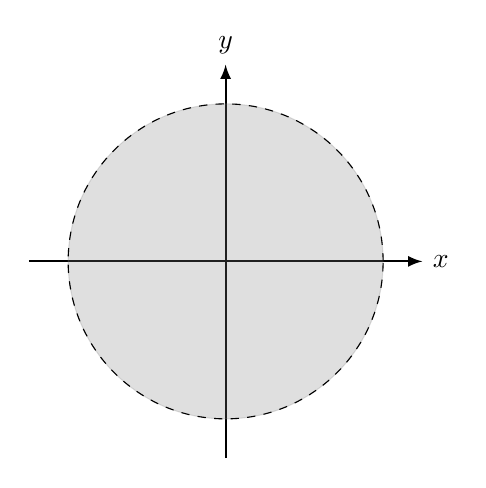
\begin{tikzpicture}
        \draw[thick,-latex] (-2.5,0) -- (2.5,0) node[right] {$x$};
        \draw[thick,-latex] (0,-2.5) -- (0,2.5) node[above] {$y$};
        \filldraw[gray,opacity=0.25] (0,0) circle (2cm);
        \draw[dashed] (0,0) circle (2cm);
    \end{tikzpicture}
    } \hfill
    \subfloat[]{
    \includegraphics[width=0.46\textwidth]{Images/Capitulo1/Esfera.pdf}
    }
    \caption{Las bolas de radio $r$ con centro en el origen en $\RR[2]$ y en $\RR[3]$ respectivamente}
\end{figure}

\begin{definition}
    Con base en lo anterior, dado $\mathbf{x}_0 \in \RR[n]$ y $r > 0$, definimos bola abierta de radio $r > 0$ con centro en $\mathbf{x}_0 \in \RR[n]$ como
    $$B(\mathbf{x}_0, r) = \left\{ \mathbf{x} \in \RR[n] \mid d(\mathbf{x}, \mathbf{x}_0) < r \right\}$$
    y definimos la bola cerrada de radio $r > 0$ con centro en $\mathbf{x}_0 \in \RR[n]$ como
    $$\overline{B(\mathbf{x}_0, r)} = \left\{ \mathbf{x} \in \RR[n] \mid d(\mathbf{x}, \mathbf{x}_0) < r \right\}$$
\end{definition}

\newpage

En otras palabras, la esfera es la cáscara y la bola es la región que se encuentra dentro de la cáscara. La bola abierta consiste en la región situada dentro de la cáscara sin incluir la cáscara en sí. La bola cerrada está formada por la región contenida dentro de la cáscara y por la cáscara misma.

Así, dado un conjunto $A \subset \RR[n]$, podemos clasificar a todos los puntos de $\RR[n]$ en términos de su “localización” con respecto a dicho conjunto, en donde por localización nos referimos a algo más profundo que el simple concepto de pertenencia. A fin de precisar esta idea de localización con respecto a un conjunto $A$, recurriremos a la figura \ref{fig:clasificacion_de_puntos} en $\RR$.
\begin{figure}[h!]
    \centering
    \subfloat[Punto interior]{
    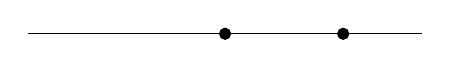
\begin{tikzpicture}
        \draw (0,0) -- (5,0);
        \filldraw (2.5,0) circle (2pt);
        \filldraw (4,0) circle (2pt);
    \end{tikzpicture}
    } \hfill
    \subfloat[Punto de adherencia]{
    \begin{tikzpicture}
        \draw (0,0) -- (5,0);
        \filldraw (5,0) circle (2pt);
    \end{tikzpicture}
    } \\
    \subfloat[Punto frontera]{
    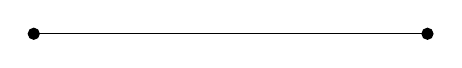
\begin{tikzpicture}
        \draw (0,0) -- (5,0);
        \filldraw (0,0) circle (2pt);
        \filldraw (5,0) circle (2pt);
    \end{tikzpicture}
    } \hfill
    \subfloat[Punto de acumulación]{
    \begin{tikzpicture}
        \draw (0,0) -- (4,0);
        \filldraw (5,0) circle (2pt);
    \end{tikzpicture}
    }
    \caption{Las diferentes localizaciones que puede tener un punto de $\RR[n]$ con respecto de un conjunto $A$}
    \label{fig:clasificacion_de_puntos}
\end{figure}
\begin{enumerate}[label=\alph*)]
    \item Un punto interior en un conjunto es aquel que tiene un entorno (una vecindad) completamente contenido dentro del conjunto. Es decir, si tomas un punto dentro del conjunto, puedes encontrar una pequeña esfera alrededor de ese punto que también está completamente dentro del conjunto.
    \item Un punto de adherencia de un conjunto es aquel alrededor del cual se pueden encontrar puntos del conjunto, dentro de cualquier entorno, incluido el propio punto. En otras palabras, un punto de adherencia puede ser tanto un punto del conjunto como un punto límite del conjunto.
    \item Un punto frontera de un conjunto es aquel que no es ni un punto interior ni un punto exterior del conjunto. Esto significa que cualquier entorno alrededor de un punto frontera contendrá puntos tanto dentro como fuera del conjunto.
    \item Un punto de acumulación de un conjunto es aquel alrededor del cual se pueden encontrar infinitos puntos del conjunto, dentro de cualquier entorno. Es decir, aunque el punto de acumulación en sí mismo no necesariamente pertenece al conjunto, existen puntos del conjunto arbitrariamente cercanos a él.
\end{enumerate}

\begin{observation}
    Se puede generalizar lo expuesto anteriormente para aplicarlo a un conjunto arbitrario $X$, en lugar de restringirse únicamente al espacio $\mathbb{R}^n$.
\end{observation}

\begin{example}
    Represente la bola siguiente utilizando la métrica $d_1$:
    $$B_{d_1} \big( (0, 0), 1 \big)$$
    \solucion Para trazar la bola anterior en el gráfico, es necesario observar que
    \begin{align*}
        (x, y) \in B_{d_1} \big( (0, 0), 1 \big) & \Longleftrightarrow d_1 \big( (0, 0), 1 \big) < 1 \\
        & \Longleftrightarrow \| (x, y) - (0, 0) \|_1 < 1 \\
        & \Longleftrightarrow \| (x, y) \|_1 < 1 \\
        & \Longleftrightarrow |x| + |y| < 1
    \end{align*}
    Por lo tanto, la representación gráfica de esta bola está dada por la figura \ref{fig:bola1}.
    \sideFigure[\label{fig:bola1}]{
    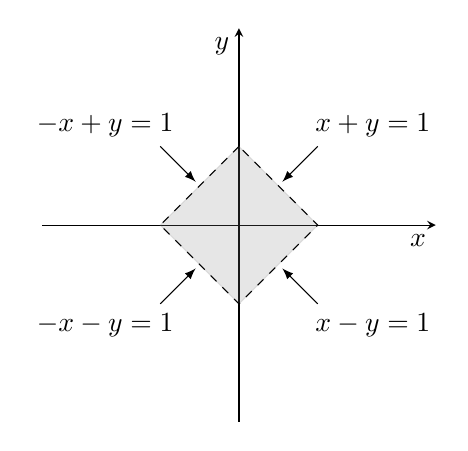
\begin{tikzpicture}
        \draw[-stealth] (-2.5,0) -- (2.5,0) node[below left] {$x$};
        \draw[-stealth] (0,-2.5) -- (0,2.5) node[below left] {$y$};
        \filldraw[gray,opacity=0.2] (0,1) -- (-1,0) -- (0,-1) -- (1,0) -- cycle;
        \draw[dash pattern=on 3pt off 3pt] (0,1) -- (-1,0) -- (0,-1) -- (1,0) -- cycle;
        \draw[latex-] (0.55,0.55) -- (1,1) node[above,xshift=0.7cm] {$x + y = 1$};
        \draw[latex-] (-0.55,0.55) -- (-1,1) node[above,xshift=-0.7cm] {$- x + y = 1$};
        \draw[latex-] (-0.55,-0.55) -- (-1,-1) node[below,xshift=-0.7cm] {$- x - y = 1$};
        \draw[latex-] (0.55,-0.55) -- (1,-1) node[below,xshift=0.7cm] {$x - y = 1$};
    \end{tikzpicture}
    }
\end{example}

\begin{example}
    Represente la bola siguiente utilizando la métrica $d_{\infty}$:
    $$B_{d_{\infty}} \big( (0, 0), 1 \big)$$\newpage\sideFigure[\label{fig:bola2}]{
    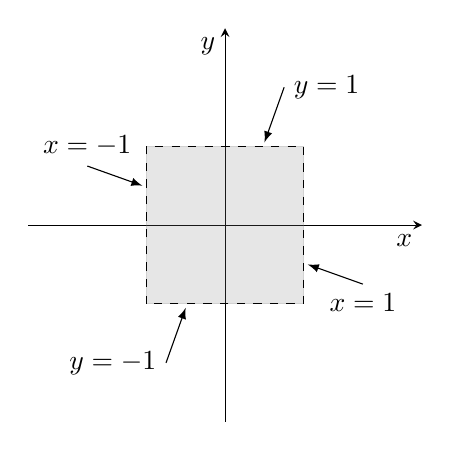
\begin{tikzpicture}
        \draw[-stealth] (-2.5,0) -- (2.5,0) node[below left] {$x$};
        \draw[-stealth] (0,-2.5) -- (0,2.5) node[below left] {$y$};
        \filldraw[gray,opacity=0.2] (-1,-1) rectangle (1,1);
        \draw[dash pattern=on 3pt off 3pt] (-1,-1) rectangle (1,1);
        \draw[latex-] (0.5,1.05) -- (0.75,1.75) node[right] {$y = 1$};
        \draw[latex-] (-0.5,-1.05) -- (-0.75,-1.75) node[left] {$y = - 1$};
        \draw[latex-] (1.05,-0.5) -- (1.75,-0.75) node[below] {$x = 1$};
        \draw[latex-] (-1.05,0.5) -- (-1.75,0.75) node[above] {$x = - 1$};
    \end{tikzpicture}
    }
    \solucion Para trazar la bola anterior en el gráfico, es necesario observar que
    \begin{align*}
        (x, y) \in B_{d_{\infty}} \big( (0, 0), 1 \big) & \Longleftrightarrow d_{\infty} \big( (0, 0), 1 \big) < 1 \\
        & \Longleftrightarrow \| (x, y) - (0, 0) \|_{\infty} < 1 \\
        & \Longleftrightarrow \| (x, y) \|_{\infty} < 1 \\
        & \Longleftrightarrow \max \left\{ |x| + |y| \right\} < 1
    \end{align*}
    Es difícil graficar la anterior expresión, así que procedamos por casos
    \begin{enumerate}[label=\roman*)]
        \item Si $\max \left\{ |x|, |y| \right\} = |y|$, entonces $|x| \leq |y| = 1$; por consiguiente, $y = \pm 1$. Si $y = 1$, entonces $|x| \leq 1$, lo que implica que $-1 \leq x \leq 1$. De manera similar, si $y = -1$, entonces $|x| \leq -1$, lo que implica que $-1 \leq x \leq 1$.
        \item Si $\max \left\{ |x|, |y| \right\} = |x|$, entonces $|y| \leq |x| = 1$; por consiguiente, $x = \pm 1$. Si $x = 1$, entonces $|y| \leq 1$, lo que implica que $-1 \leq y \leq 1$. De manera similar, si $x = -1$, entonces $|y| \leq -1$, lo que implica que $-1 \leq y \leq 1$.
    \end{enumerate}
    Por lo tanto, la representación gráfica de esta bola está dada por la figura \ref{fig:bola2}.
\end{example}

\begin{example}
    Represente la bola siguiente utilizando la métrica $d_{2}$:\sideFigure[\label{fig:bola3}]{
    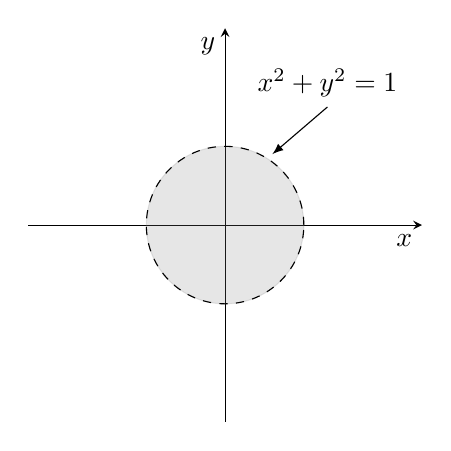
\begin{tikzpicture}
        \draw[-stealth] (-2.5,0) -- (2.5,0) node[below left] {$x$};
        \draw[-stealth] (0,-2.5) -- (0,2.5) node[below left] {$y$};
        \filldraw[gray,opacity=0.2] (0,0) circle (1cm);
        \draw[dash pattern=on 3pt off 3pt] (0,0) circle (1cm);
        \draw[latex-] (0.6,0.9) -- (1.3,1.5) node[above] {$x^2 + y^2 = 1$};
    \end{tikzpicture}
    }
    $$B_{d_{2}} \big( (0, 0), 1 \big)$$
    \solucion Para trazar la bola anterior en el gráfico, es necesario observar que
    \begin{align*}
        (x, y) \in B_{d_2} \big( (0, 0), 1 \big) & \Longleftrightarrow d_2 \big( (0, 0), 1 \big) < 1 \\
        & \Longleftrightarrow \| (x, y) - (0, 0) \|_2 < 1 \\
        & \Longleftrightarrow \| (x, y) \|_2 < 1 \\
        & \Longleftrightarrow \sqrt{x^2 + y^2} < 1
    \end{align*}
    Por lo tanto, la representación gráfica de esta bola está dada por la figura \ref{fig:bola3}.
\end{example}

\subsection{Conjuntos abiertos y cerrados}

\begin{observation}
    Diremos que un conjunto es abierto si para toda $\mathbf{y} \in B(\mathbf{x}, r)$, existe $r_0 = \dfrac{r - d(\mathbf{y}, \mathbf{x})}{2} > 0$ tal que $B(\mathbf{y}, r_0) \subset B(\mathbf{x}, r)$. Geométricamente,
    \begin{center}
        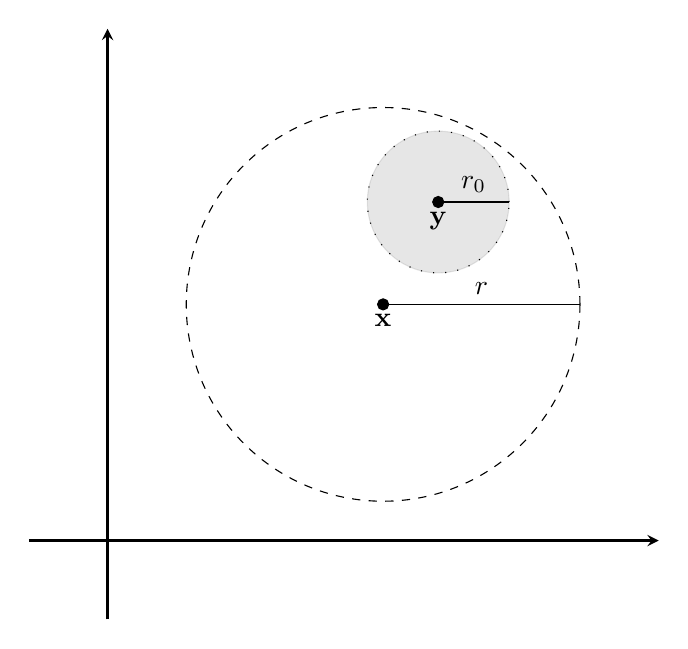
\begin{tikzpicture}
            \draw[dash pattern=on 3pt off 3pt] (0,0) circle (2.5cm);
            \filldraw[gray,opacity=0.2] (0.7,1.3) circle (0.9cm);
            \draw[loosely dotted] (0.7,1.3) circle (0.9cm);
            \draw (0,0) -- (2.5,0) node[midway,above] {$r$};
            \draw (0.7,1.3) -- (1.6,1.3) node[midway,above] {$r_0$};
            \filldraw (0,0) circle (2pt) node[below] {$\mathbf{x}$};
            \filldraw (0.7,1.3) circle (2pt) node[below] {$\mathbf{y}$};
            \draw[-stealth,thick] (-3.5,-4) -- (-3.5,3.5);
            \draw[-stealth,thick] (-4.5,-3) -- (3.5,-3);
        \end{tikzpicture}
    \end{center}
\end{observation}

\newpage

\begin{proposition}~
    \begin{enumerate}[label=\roman*.]
        \item La intersección de dos bolas es un conjunto abierto.
        \item El conjunto vacío es un conjunto abierto.
    \end{enumerate}
    \demostracion
    \begin{enumerate}[label=\roman*.]
        \item Sea $\mathbf{z} \in B(\mathbf{x}, r_1) \cap B(\mathbf{y}, r_2)$, entonces $\mathbf{z} \in B(\mathbf{x}, r_1)$ y $\mathbf{z} \in B(\mathbf{y}, r_2)$. Así, existe $r_0 > 0$ y $r_0^{*} > 0$ tal que $B(\mathbf{z}, r_0) \subseteq B(\mathbf{x}, r_1)$ y $B(\mathbf{z}, r_0^{*}) \subseteq B(\mathbf{x}, r_1)$. Sea $r_0^{**} = \min \left\{ r_0, r_0^{*} \right\}$, entonces
        $$B(\mathbf{z}, r_0^{**}) \leq B(\mathbf{z}, r_0) \quad \text{ y } \quad B(\mathbf{z}, r_0^{**}) \leq B(\mathbf{z}, r_0^{*}).$$
        Por tanto, $B(\mathbf{z}, r_0^{**}) \subseteq B(\mathbf{x}, r_1) \cap B(\mathbf{y}, r_2)$, por lo que $B(\mathbf{x}, r_1) \cap B(\mathbf{y}, r_2)$ es un conjunto abierto.
        \item Supongamos que el conjunto vacío $\emptyset$ no es abierto. Entonces, existe un $\mathbf{x} \in \emptyset$ tal que para todo $r > 0$, $B(\mathbf{x}, r) \nsubseteq \emptyset$. En particular, esto implica que existe un $\mathbf{x} \in \emptyset$, lo cual es una contradicción. Por lo tanto, $\emptyset$ es un conjunto abierto.
    \end{enumerate}
\end{proposition}